
\subsection{Revolutionary Science}

\cite{kuhn2012} posits that scientific knowledge advances through periods of incremental progress punctuated by abrupt, revolutionary changes in understanding. According to Kuhn, during normal science, scientists work within an accepted paradigm, which is a set of assumptions, concepts, and methods that define a scientific discipline at a given time. Scientists in a paradigm share a common language, a set of beliefs, and a set of practices that enable them to conduct research and generate new knowledge within the paradigm.

However, as anomalies and inconsistencies between what the models predict and what is observed accumulate within the paradigm, scientists may begin to question its validity, and a crisis may emerge. During this crisis, scientists may propose new theories and methods that challenge the existing paradigm. If a new theory is accepted, it may eventually replace the old paradigm, leading to a scientific revolution.

\subsection{Fractal Science}

\citeauthor{abbott2001}'s \citeyearpar{abbott2001} fractal division of disciplines is a model that suggests that any discipline can be divided into smaller sub-disciplines, which in turn can be further divided into smaller sub-sub-disciplines, and so on, creating a fractal-like structure.

Figure \ref{fig:fractal_distinctions} (p. 14)

\begin{figure}[H]
	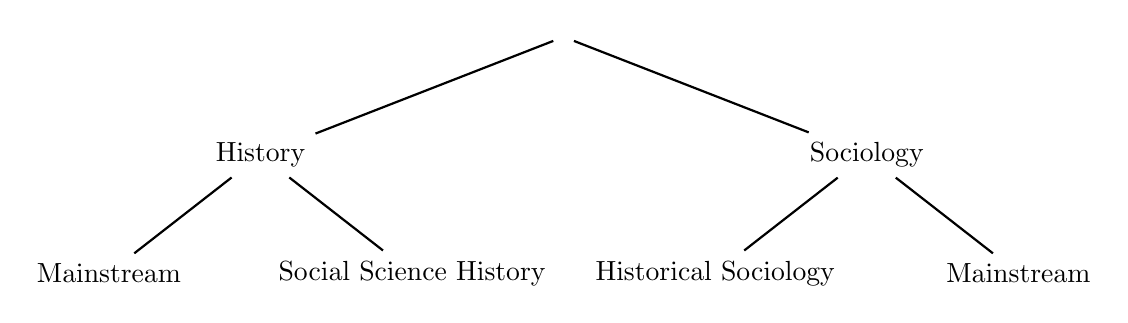
\begin{tikzpicture}[thick,level/.style={sibling distance=77mm/#1}]
	\node [] (r) {}
	  child {
	    node [] (a) {History}
	    child {
	      node [] {Mainstream}
	    }
	    child {
	      node [] {Social Science History}
	    }
	  }
	  child {
	    node [] {Sociology}
	    child {
	      node [] {Historical Sociology}
	    }
	    child {
	      node [] {Mainstream}
	    }
	  };
	\end{tikzpicture}
	\caption{Fractal Distinctions} 
	\label{fig:fractal_distinctions}
\end{figure}

\subsection{High Consensus, Rapid Discovery Science}

\cite{collins1994} posits that achieving high levels of consensus and rapid scientific discovery in science research relies on the use of research technologies and techniques that generate consistent, observable, and reliable data, resulting in a high degree of reproducibility. As a result, conflict and disagreement are limited to the frontiers of research. 

The natural sciences have experienced high levels of consensus and rapid scientific discovery since the post-scientific revolution of the 1600s, but this has not been solely due to empiricism, mathematization, measurement precision, or the experimental method that existed before this era. Instead, the distinguishing feature of this time period has been the creation of research technologies that facilitate the production of new data and observations.

The social sciences face obstacles not solely due to a lack of common ideas, as Kuhn suggests, but also from a dearth of technologies that produce consistent data and results: "The most glaring lack within social science is a self-generating lineage of research technologies" (p. 165).

\subsection{Attention in Science}

The "Law of Small Numbers" is a concept first introduced by \cite{collins1998}, which is based on the idea of a "limited attention space" which sets an upper bound on the possible number of subfields in a field. This concept has been further developed by other researchers, with Price (1986) suggesting that the number of items that can be held in attention is around five, while Collins himself revised this number to seven in 1994. In other words, the "Law of Small Numbers" is analogous to a carrying capacity.

A binomial distribution can be used to describe the number of groups competing for attention in situations where there are two possible outcomes for each group (i.e. success or failure in acquiring the resource). The binomial distribution can be used to calculate the probability of a given number of groups successfully acquiring the resources. For example, if there are 10 groups competing for a finite number of resources, the binomial distribution can be used to calculate the probability of each possible number of groups (from 0 to 10) successfully acquiring the resources. I expect to observe a binomial distribution with a mode of anywhere between 1 and 7 for the number of subfields in a field, but most likely between 5 and 7.

\subsection{Phases of Science}

\cite{mullins1973} proposed a model for the development of scientific fields that incorporates elements from both the "invisible college" \citep{desollaprice1966, crane1969, crane1972, paisley1972} and "scientific revolutions" \citep{kuhn2012}. According to Mullins, the development of scientific fields is determined by the interactions and competition between different "theory groups", which are networks of scientists who share similar ideas and interests.

Mullin's model consists of four stages, which are as follows:

\begin{enumerate}

\item Normal: In the normal stage of theory group development, the communication network among researchers is loosely coupled, meaning that there is only a weak connection between the different researchers within the group. This stage is characterized by low clustering and density, and individual researchers are largely focused on solving specific problems within the field. This stage is similar to what Kuhn (1962) referred to as the "puzzle-solving" or "paradigmatic" phase of scientific development, in which researchers are largely focused on applying established theories and methods to the study of specific phenomena. In this phase, there is little attention to or interest in alternative paradigms or theories, and the focus is on making incremental advances within the existing framework.

\item Network: In the network stage of theory group development, the patterns of communication among researchers begin to change due to the emergence of one or more influential ideas or theories that attract the attention of multiple researchers. This leads to a shift in the focus of the group and the development of a consensus among its members, which allows for the creation of an alternative paradigm or approach to the problem they are studying. As the group becomes more focused and cohesive, communication within the group increases, while communication with external researchers or other groups declines. In this phase, the group's success in advancing their ideas and theories is crucial for maintaining its growth and attracting new members.

\item Cluster: The third stage of theory group development, known as the cluster phase, is characterized by the emergence of a power-law distribution of communication ties among researchers. In this phase, clusters of researchers typically form around the most productive or influential members of the group, who can often be found in one or a few institutions. This creates a positive feedback loop, where the ideas and theories of the most productive researchers are reinforced and strengthened by the input and support of the other members of the cluster. This can lead to the institutionalization of the group and its ideas, as the cluster becomes increasingly recognized and respected within the broader field. As the group's ideas and theories evolve, they may also begin to diverge from the established concepts and theories of the parent discipline, reflecting the group's growing focus and specialization. According to Mullin (1973), the degree of divergence from the parent field is a function of the group's size and isolation, with larger and more isolated groups being more likely to develop their own distinct paradigms and theories. 

At this point, the group can take one of two possible trajectories, depending on the parent discipline's reaction to the group's ideas. If the parent discipline rejects or ignores the group's ideas, the group may become isolated and continue to develop their ideas independently, remaining in the cluster stage. This is often referred to as a "revolutionary" trajectory, as the group is effectively challenging the existing paradigms and theories of the parent discipline. On the other hand, if the parent discipline adopts or diffuses the group's ideas, the group may become integrated into the broader field and recognized as an "elite" group. In this case, the group's ideas may become mainstream and widely accepted within the parent discipline.

\item Speciality: The final stage of theory group development, known as the specialty phase, is only reached by "elite" groups whose ideas are adopted and diffused by the parent discipline. In this phase, the group's members may begin to scatter and move to different institutions or locations, weakening the connections within the group and enabling the diffusion of their ideas to a wider audience. This process of scattering and diffusion can lead to the routinization and institutionalization of the group's ideas, as they become integrated into the broader field of knowledge and accepted as a new paradigm or approach. Over time, the dense network of communication within the group may begin to loosen again, returning to the more loosely-coupled, normal pattern of communication seen in the earlier stages of theory group development.

\end{enumerate}

The transition between the different phases of theory group development is not guaranteed, and groups may fail or die off before reaching the later stages. The success of a group and its ability to advance through the different phases is contingent on a number of factors, including its ability to grow and attract new members at a faster rate than alternative groups. This in turn is dependent on factors such as the group's apparent success in advancing their ideas, the presence of strong intellectual leaders within the group, the support and recognition of the broader community, the availability of research centers and materials to support the group's work, and the output of textbooks and other materials that can help to promote and disseminate the group's ideas.



